\documentclass[11pt]{article}
\usepackage[utf8]{inputenc}
\usepackage[T1]{fontenc}
\usepackage{amsmath}
\usepackage{amsfonts}
\usepackage{amssymb}
\usepackage[version=4]{mhchem}
\usepackage{stmaryrd}
\usepackage{graphicx}
\usepackage[export]{adjustbox}
\graphicspath{ {./images/} }

\begin{document}
Introduction to Collateralized Debt Obligations

This lesson introduces the concept of a collateralized debt obligation. A collateralized debt obligation (CDO) applies the concept of structuring to cash flows from a portfolio of debt securities into multiple claims; these claims are securities and are referred to as tranches.

Of course, in practice, traditional operating corporations and other applications of structuring are usually financed with numerous classes of securities. Major corporations usually have multiple types of debt (accounts payable, short-term credit facilities, senior bonds, junior bonds) or preferred stock. Some corporations even have multiple types of equity, which may differ in terms of voting rights or liquidity. The concept of multiple security types also extends beyond the traditional operating firm to such applications as multiple commercial mortgages on a single property, multiple types of securities as sources of capital for closed-end funds, and multiple bond issues for various levels of government.

The use of structuring to create multiple security types in alternative investing centers on CDOs. The concept of a CDO is relatively new, but in just a few decades, CDOs have become an important part of financial institutions, markets, and activities. As previously illustrated in the case of mortgages, the structures are quite simple. In its simplest form, a CDO is a collection or portfolio of assets financed with multiple securities (or tranches) that differ in regard to their seniority. This section provides an introduction to the structuring of cash flows for default risk. The session, CDO Structuring of Credit Risk provides a more detailed discussion of various types of CDO structures, purposes for their establishment, and their common applications.

\section*{A Stylized CDO}
The next exhibit, Simplified CDO Structure illustrates the concept of a CDO that is being used to structure the cash flows and default risk from a portfolio of high-yield bonds. There are $\$ 100$ million of high-yield bonds on the left-hand side of the next exhibit that serve as the assets or collateral portfolio (or pool) for the structure. These bonds generate cash flows in the form of coupon payments and principal payments. The bond portfolio can also generate losses from events such as defaults in the bonds and from profits or losses from trading activity. On the right-hand side of the structure are the various classes of securities (or tranches) that provided the financing for the portfolio and that have claims of varying seniorities to receive cash inflows.

\begin{center}
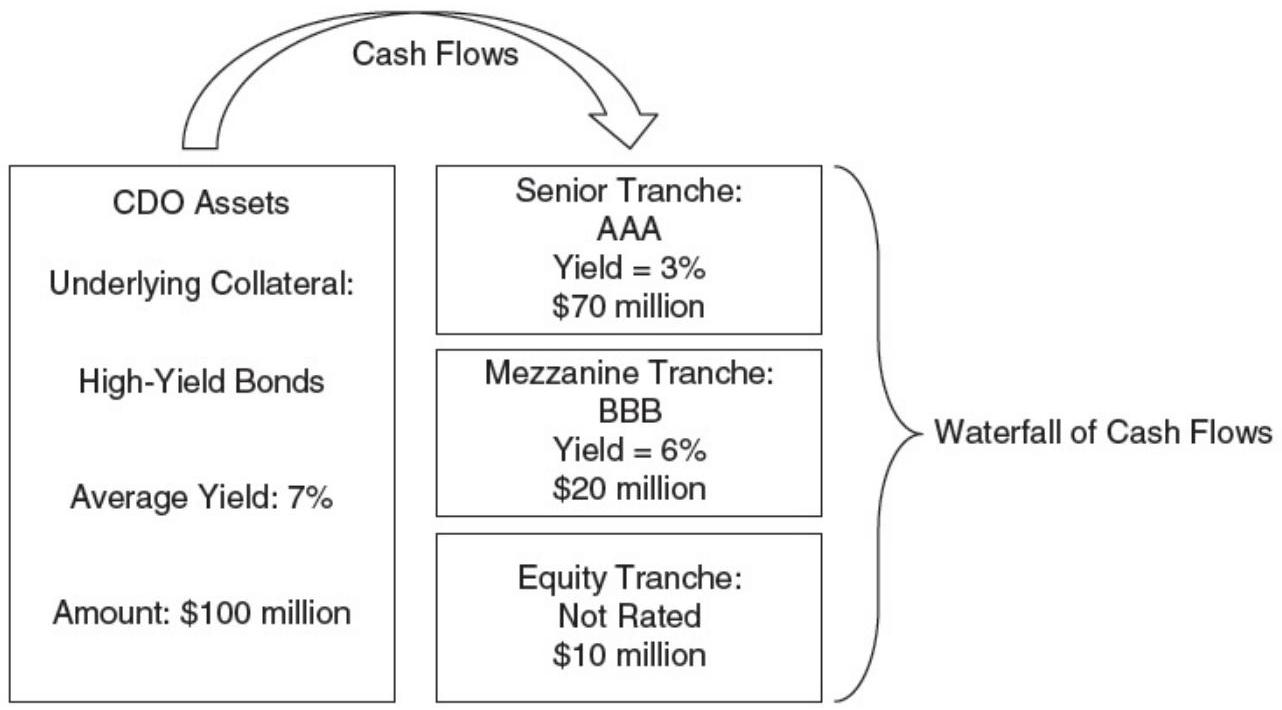
\includegraphics[max width=\textwidth]{2024_04_09_feb3065896628696873eg-2}
\end{center}

\section*{Simplified CDO Structure}
The cash flows from the collateral pool of assets are distributed using a waterfall approach somewhat analogous to that discussed in the session, The Environment of Alternative Investments for limited partnerships. Without any defaults, the assets should generate $\$ 7$ million in coupon income, found as the product of the asset size ( $\$ 100$ million) and the average coupon of the assets (7\%). The first priority of the cash flows is to meet direct expenses and fees for the operation and management of the CDO. For simplicity, this example ignores the expenses and fees.

After expenses and fees, the cash flows are distributed to the various tranches in order of their seniority. The senior tranche is a tranche with the first or highest priority to cash flows in the structured product. In this case, the senior tranche is owed the first $\$ 2.1$ million per year in coupon income, found as the product of its size ( $\$ 70$ million) and the coupon rate (3\%). A mezzanine tranche is a tranche with a moderate priority to cash flows in the structured product and with lower priority than the senior tranche. In this case, the mezzanine tranche is owed $\$ 1.2$ million per year after the senior tranche has been paid. The equity tranche has lowest priority and serves as the residual claimant. In this case, the equity tranche has claim to the remaining $\$ 3.7$ million.

\section*{Default Risk and CDO Cash Flows}
The previous numerical example ignored defaults in the bond portfolio. However, this CDO contains bonds subject to substantial credit risk, since they are below investment grade (i.e., are rated BB or lower), and therefore it is reasonable to expect defaults. When collateral assets default, the order of the waterfall reverses relative to the order for receiving cash flows, such that the lowest seniority tranches experience the losses first. The losses from asset defaults are posted against the lowest remaining tranche until that tranche is wiped out, at which point the losses are posted against the next lowest seniority tranche. For example, if $\$ 11$ million of assets completely defaulted (i.e., experienced no recovery), the equity tranche would be wiped out, and the notional principal of the mezzanine tranche would be reduced from $\$ 20$ million to $\$ 19$ million. If $\$ 11$ million of assets defaulted with $60 \%$ recovery, the assets would drop by only $\$ 4.4$ million, causing loss only to the equity tranche.

Note that defaults in the CDO's collateral portfolio reduce both the left and right sides of Simplified CDO Structure exhibit. The assets are reduced in size and in annual income. The aggregated tranches are reduced in size by reducing the tranches, starting with the lowest-seniority tranche. As the debt tranches are reduced in notional principal, their claim to coupon income is reduced. Thus, if the mezzanine tranche in the example is reduced from $\$ 20$ million to $\$ 19$ million, the annual coupons owed to the mezzanine tranche holders would fall from $\$ 1.20$ million to $\$ 1.14$ million.

\section*{Attachment Points, Detachment Points, Calls, and Puts}
Note that the $20 \%$ of the structure in Simplified CDO Structure exhibit that is represented by the mezzanine debt tranche lies between the $70 \%$ financed by senior debt and the $10 \%$ financed by the most junior tranche (the equity tranche). As losses to the collateral pool are experienced due to defaults in the portfolio of bonds, the first $10 \%$ of the losses are applied against the equity tranche, and the last $70 \%$ are applied against the senior tranche. Thus, the losses to the mezzanine tranche begin when $10 \%$ of the collateral assets have been lost to default and end when $30 \%$ of the collateral assets have been lost to default and the mezzanine tranche is eliminated.

The first percentage loss in the collateral pool that begins to cause reduction in a tranche is known as the lower attachment point, or simply the attachment point. The higher percentage loss point at which the given tranche is completely wiped out is known as the upper attachment point, or the detachment point. Thus, the mezzanine tranche in the simplified example has a lower attachment point of $10 \%$ and an upper attachment point of $30 \%$. Each tranche is often identified using these points, such that the mezzanine tranche in the example might be described as being a 10\%/30\% mezzanine tranche.

The risks and payoffs to the most senior and most junior tranches in a CDO can be viewed using positions in either a call or a put. Similarly, the structural credit risk model discussed earlier in this session expressed the positions of equity holders and debt holders in the traditional capital structure of an operating firm as being synonymous with call options or put options. The senior debt tranche in the example illustrated in Simplified CDO Structure exhibit may be viewed in the structural model as either a covered call or a riskless bond with a short put position on the assets. Similarly, the equity tranche can be viewed in the structural model as either a long position in a call option or a financed long position in the assets with a long put position.

\section*{Option Collars Are Similar to a Mezzanine Tranche}
The economic essence of the $10 \% / 30 \%$ mezzanine tranche in the previous section was that the mezzanine tranche benefits from investment success in the collateral pool within the range of the assets retaining $70 \%$ of their value to $90 \%$ of their value. If the assets fall below $70 \%$ of their original value, the mezzanine tranche is wiped out, and the senior tranche begins bearing losses. If the assets retain $90 \%$ or more of their value, the value in excess of $90 \%$ benefits the equity tranche. Whereas the most senior and most junior tranches can be viewed with single positions in options, mezzanine tranches can be viewed with option strategies involving two options. There are three theoretically equivalent option strategies that mimic a mezzanine tranche, each involving two options: a collar position, a bull call spread, and a bull put spread.

Let's begin with viewing a mezzanine tranche as a collar position. As detailed in the session, Derivatives and Risk-Neutral Valuation, a collar combines a long position in an asset with a short position in a call option and a long position in a put option. In this example, the long position in the asset is $70 \%$ financed. Both options are on the same asset and have the same expiration date, but the call option has a higher strike price than the put option. Owning a mezzanine tranche is like owning the collateral asset, owning a put option that places a floor on losses when the assets are below a particular amount ( $70 \%$ in the example), and writing a call option that places a cap on profits when the assets remain at or above a particular amount ( $90 \%$ in the example).

Thus, the mezzanine tranche in Simplified CDO Structure may be described as a collar with a financed position in the collateral pool, a long position in a put at the lower attachment point, and a short position in a call at the upper attachment point. The mezzanine tranche is net long between $\$ 70$ million and $\$ 90$ million in assets, with profits limited at and above $\$ 90$ million in assets, and losses limited at and below $\$ 70$ million in assets.

\section*{Mezzanine Tranches and Option Spreads}
As noted in the Derivatives and Risk-Neutral Valuation session, a collar position has the same payout as a bull option spread; thus, a mezzanine tranche may be mimicked with a bull option spread. A bull spread combines a long and short position in either calls or puts, which differ only with regard to strike prices. A bull spread involves a long position in the option with the lower strike price and a short position in the option with the higher strike price. The bull spread offers positively correlated performance between the strike prices, places a cap on profits at the higher strike price, and places a floor on losses at the lower strike price. The top left\\
panel in the exhibit, Diagrams of Options Spreads and Combinations (in the Option Exposures lesson) illustrates the profit and loss diagram of a bull spread (as well as a collar position).

Bull spreads may be formed with two calls or two puts. A bull call spread has two calls that differ only by strike price, in which the long position is in the lower strike price and the short position is in the higher strike price. A bull put spread has two puts that differ only by strike price, in which the long position is in the lower strike price and the short position is in the higher strike price. Bear spreads are the mirror positions. The underlying assets to the options are the collateral pool.

A bull call spread that mimics the $10 \% / 30 \%$ mezzanine tranche in the example contains a long call option with a strike price of $\$ 70$ million and a short call option with a strike price of $\$ 90$ million. The bull call spread, like the mezzanine tranche, benefits from increases in the collateral pool between $\$ 70$ million and $\$ 90$ million. The analogous bull spread with put options is long a put option with a strike price of $\$ 70$ million and short a put option with a strike price of $\$ 90$ million. In summary, a mezzanine tranche can be viewed as a bull call spread or a bull put spread on the CDO's portfolio.

It may appear counterintuitive that a bull option spread has a long position in the option with the lower strike price and a short position in the option with the higher strike price regardless of whether the spread uses calls or puts. However, note that in the previous example, when the structure's assets (i.e., the collateral pool) are worth $\$ 80$ million, the bull call spread has only one option that is in-the money (a long call), and the bull put spread has only one option that is in-the-money (a short put). Both a long call and a short put are bullish positions.


\end{document}